Vi valgte at vores system skal kunne klare at blive slukket og tændt uden at det ville miste alle dataerne omkring vores udtags tændt/slukket status, adresser, navne og brugeren telefon nummer. Derfor besluttede vi at vi skulle have en klasse på PCen som kunne gemme og loade disse dataer. Det står klassen Hukommelse for.
\medskip

Klassen hukommelse læser og redigere i en text fil hver gang der sker ændringer. Når den læser text filen skriver den hver linje ind på en plads i en vector som kan indeholde strings. Linje 1 i text filen kommer altså til at stå på plads nr 0 i vectoren osv.

\medskip
Telefon nummeret står altid på den første linje i text filen og ligger altså altid på plads nr 0 i vectoren. Enhederne har 3 parametre som vi gerne vil gemme. Deres adresse, navn og status. De bliver gemt i den ordre, dvs at adressen på den første enhed ligger på plads nr 1 (vectornavn[1]) hvorefter navn står på nr 2 og status på nr 3.\\

\begin{figure}[!htb]
     {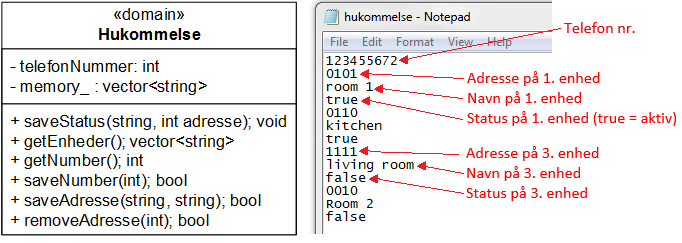
\includegraphics[width=\textwidth]{billeder/uml/PC_dataview}}
     \caption{Hukommelses header og udklip af text filen den gemmer i}
     \label{fig:PC_dataview}
\end{figure}